

%\subsection{Reversed Entropy Policy Mirror Descent}
\section{Reversed Entropy Policy Mirror Descent}
\label{subsec:repmd}

We now introduce two modifications to PMD that overcome 
its aforementioned deficiencies.
These two modifications lead to our main proposed algorithm,
Reversed Entropy Policy Mirror Descent (REPMD),
which retains desirable theoretical properties while achieving
vastly superior performance to PMD in practice.
%(We consider some additional refinements to REPMD in the next section.)

The first modification is to add an additional entropy regularizer
to the Lift Step,
to improve the exploration behavior. %of the algorithm. 
The second modification is to use a reversed, \emph{mean seeking} direction
of the KL divergence in the Project Step.
In particular, the REPMD algorithm solves the following 
alternating
optimization problems to update the policy $\pi_{\theta_{t+1}}$
at each iteration:
%
{\small
\begin{equation}
\label{eq:repmd}
\begin{split}
&\text{\bf (Project)} \quad  \argmin\limits_{\pi_\theta \in \Pi}{\KL(\bm{ \bar{\pi}_{\tau,\tau^{\prime}}^* \| \pi_\theta }) }, \\
&\text{\bf (Lift)} \quad \text{where}\ \ \bar{\pi}_{\tau,\tau^{\prime}}^*  =  \argmax\limits_{\pi \in \Delta}{ \ep\limits_{\rho \sim \pi}{  r(\rho) }} \\
&\qquad \qquad \qquad \qquad \qquad \quad {{ - \tau \KL(\pi \| \pi_{\theta_t}) + \bm{\tau^{\prime} \cH(\pi)} }}.
\end{split}
\end{equation}
}
%

The idea of optimizing the reverse direction of KL divergence has proved
to be effective in previous work,
such as reward augmented maximum likelihood \citep{norouzi2016reward}
and UREX \citep{nachum2017improving}.
Its \emph{mean seeking} behavior further encourages exploration by the
algorithm.
As we will see in \cref{sec:experiments},
REPMD outperforms PMD significantly in experimental evaluations.

\cref{thm:monotonically_increasing_sr_property}
shows that REPMD still enjoys similar desirable properties to PMD
in the non-convex setting,
but with respect to a surrogate reward $\SR(\pi_\theta)$,
which we analyze further below.

\begin{thm}
\label{thm:monotonically_increasing_sr_property}
Let $\pi_{\theta_{t}}$ denote the policy at step $t$ of the update
sequence.
REPMD satisfies the following properties for an arbitrary parametrization of $\pi$.
\begin{enumerate}
	\item {\bf (Monotonic Improvement)} 
	%The sequence of policies learned by TRPO is guaranteed to be monotonically improved:
	If the Project Step $\KL( \bar{\pi}_{\tau,\tau^{\prime}}^* \| \pi_\theta )$ can be globally solved,
then 
	\begin{equation*}
	\SR(\pi_{\theta_{t+1}}) - \SR(\pithetat)\ge 0,
	\end{equation*}
	where
	{\small
	\begin{equation}
	\label{eq:SR}
	\SR(\pi_\theta) \triangleq (\tau + \tau^{\prime})\log{ \sum_{\rho}{ \exp\left\{ \frac{r(\rho) + \tau \log{\pi_\theta(\rho)} }{\tau + \tau^{\prime}} \right\} }}.
	\end{equation}
	}
	\item {\bf (Fixed Points)} If the Project Step is optimized by gradient descent, then the fixed points of REPMD are the 
	stationary points of $\SR(\pi_\theta)$. 
\end{enumerate}
%Theorem \ref{thm:monotonically_increasing_sr_property} guarantees the monotonic improvement on $\text{SR}(\pi)$, thus implies that 
%the fixed points of REPMD have a correspondence with the stationary point of $\text{SR}(\pi_\theta)$. \todor[]{Why?}
\end{thm}

A key question is the feasibility of solving the
Project Step to global optimality.
It is obvious that when $\pi(\theta) = \theta \in \Delta$
the Project Step is a convex optimization problem,
hence can be solved optimally.
Furthermore, as shown in \cref{prop:solvableprojection}, 
for a one-layer-softmax neural network $\pi$,
the Project Step $\KL( \bar{\pi}_{\tau,\tau^{\prime}}^* \| \pi_\theta)$
can also still be solved to global optimality,
affording a significant computational advantage over PMD.

\begin{prop}
\label{prop:solvableprojection}
Assume $\pi_\theta(s) = \softmax(\phi_s^{\top}\theta)$.
Given any $\refPi$,
the Projection Step
$\min\nolimits_{\theta \in \mathbb{R}^d}{\KL(\refPi \| \pi_\theta)}$
is a convex optimization problem in $\theta$.
\end{prop}

\subsection{Learning Algorithms}

We now provide REPMD learning algorithms.
Despite its non-convexity, the Lift Step
has an analytic solution,
{\small
\begin{equation}
	\label{eq:pitautauprime}
	\bar{\pi}_{\tau,\tau^{\prime}}^*(\rho) \triangleq \frac{\refPi(\rho) \exp\left\{ \frac{r(\rho)-\tau^{\prime} \log \refPi(\rho) }{ \tau+\tau^{\prime}} \right\}}{ \sum_{\rho^{\prime}}{\refPi(\rho^{\prime}) \exp\left\{ \frac{r(\rho^{\prime})-\tau^{\prime} \log \refPi(\rho^{\prime})}{ \tau+\tau^{\prime}} \right\} } }.
\end{equation}
}
	
The Project Step in \cref{eq:repmd}, $\min\nolimits_{\pi_\theta \in \Pi}{\KL(\bm{ \bar{\pi}_{\tau,\tau^{\prime}}^* \| \pi_\theta }) }$, can be optimized via stochastic gradient descent, given that one can sample trajectories from $\bar{\pi}_{\tau,\tau^{\prime}}^*$. To see this, note $\argmin\nolimits_{\pi_\theta \in \Pi}\KL(\bar{\pi}_{\tau,\tau^{\prime}}^* \| \pi_\theta) = \argmin\nolimits_{\pi_\theta \in \Pi} \ep_{\rho \sim \bar{\pi}_{\tau,\tau^{\prime}}^* }  - \log \pi_\theta(\rho)$. The next lemma shows that sampling from $\bar{\pi}_{\tau,\tau^{\prime}}^*$ can be done using self-normalized importance sampling \citep{owen2013monte} when it is possible to draw multiple samples from $\refPi$, following the idea of UREX \citep{nachum2017improving}.   
\begin{lem}
\label{lem:repmdgradientestimate}
Let $\omega_k = \frac{r(\rho_k) - \tau^{\prime} \log{\refPi(\rho_k)} }{\tau + \tau^{\prime}}$. Given $K$ \emph{i.i.d.} samples $\{\rho_1, \dots, \rho_K\}$ from the \emph{reference policy} $\refPi$, we have the following unbiased gradient estimator,
{\small
\begin{equation}
\label{eq:gradient_estimator}
	\nabla_{\theta} \KL(\bar{\pi}_{\tau,\tau^{\prime}}^* \| \pi_\theta)\approx -\sum\limits_{k=1}^K{ \frac{ \exp\left\{ \omega_k \right\} }{ \sum_{j=1}^K{ \exp\left\{ \omega_j \right\}}} \nabla_{\theta} \log{\pi_\theta(\rho_k)} },
\end{equation}
}
\end{lem}
Derivation for the analytic solution of the Lift Step and above Lemma as well as other implementation details can be found in \cref{appx:repmd-learning}.

\begin{algorithm}[t]
	\caption{\label{alg:repmd}  The REPMD algorithm}
	\begin{algorithmic}[1]
		\INPUT temperature parameters $\tau$ and $\tau'$, number of samples for computing gradient $K$
		\STATE Random initialized $\pi_{\theta}$
		\FOR { $t=1,2,\ldots$ }
		\STATE Set $\refPi = \pi_\theta$
		\REPEAT 
		\STATE Sample a mini-batch of $K$ trajectories from $\refPi$
		\STATE Compute the gradient according to \cref{eq:gradient_estimator}
		\STATE Update $\pi_{\theta}$ by gradient descent
		\UNTIL $t$ reaches maximum of training steps
		\ENDFOR
	\end{algorithmic}
\end{algorithm}

%\subsubsection{Behavior of $\SR(\pi)$}
\subsection{Behavior of $\SR(\pi_\theta)$}
\label{subsec:sr}

\cref{thm:monotonically_increasing_sr_property} only establishes
desirable properties for REPMD with respect to $\SR(\pi_\theta)$,
but not necessarily $r(\rho)$.
In this section we present theoretical and empirical evidence that
$\SR(\pi_\theta)$ is a reasonable surrogate 
that can provide good guidance for learning,
even when targeting desirable behavior with respect to $r(\rho)$.
In fact, by properly adjusting the two temperature parameters $\tau$ and
$\tau^{\prime}$ in REPMD,
the resulting surrogate objective $\SR(\pi_\theta)$
recovers existing performance measures.

\begin{prop}
\label{prop:sr}
$\SR(\pi_\theta)$ satisfies the properties:
\begin{enumerate}[label=(\roman*)]
	\item  $\SR(\pi_\theta) \to \max_{\rho}{r(\rho)}$, as $\tau \to 0, \tau^{\prime} \to 0$.
	\item $\SR(\pi_\theta) \to \ep_{\rho \sim \pi_\theta}{r(\rho)}$, as $\tau \to \infty, \tau^{\prime} \to 0$. 
\end{enumerate}	
\end{prop}

\begin{remk}
Note that $\text{SR}(\pi_\theta)$ also resembles the 
``softmax value function'' in value based RL
\citep{nachum2017bridging,haarnoja2018soft,ding2017cold}.
The standard softmax value can be recovered by
$\text{SR}(\pi_\theta)$ as a special case when $\tau = 0$ or $\tau'=0$. 
	%\todor[]{But \cref{prop:sr} says that $SR(\pi)$ converges to $max_\rho$ when $\tau$ and $\tau^\prime$ are 0?}
\end{remk}

According to \cref{prop:sr}, one should gradually decrease $\tau^{\prime}$
to reduce the level of exploration as sufficient reward landscape information
is collected during the learning process.
Different choices can be made for $\tau$,
depending on the policy constraint set $\Pi$.
Given $\tau^{\prime} \to 0$ and a sufficiently explored reward landscape,
the resulting unconstrained policy must satisfy
$\bar{\pi}_{\tau,\tau^{\prime}}^* \to \pi^*$ as $\tau \to 0$,
where $\pi^*$ is the globally optimal deterministic policy. 
Therefore, in the Project Step, $\pi_\theta$ is obtained by directly
projecting $\pi^*$ into $\Pi$.
When the policy constraint $\Pi$ has nice properties
that support good behavior of KL projection,
such as convexity,
$\pi_\theta$ will achieve good performance.
However, in practice, $\Pi$ is typically non-convex,
and setting $\tau \to 0$ might not work very well,
since directly projecting $\pi^*$ into $\Pi$ will not always lead to
a $\pi_\theta$ with large expected reward.



On the other hand, as $\tau \to \infty$,
the stationary point of $\SR(\pi_\theta)$ will approach the
stationary point of $\sum_{\rho}{ \pi_\theta(\rho) r(\rho) }$.
\cref{fig:srsimulation} shows the a simulation
investigating the behavior of $\SR(\pi_\theta)$ for different $\tau$.
Note that there is a poor local maximum for $\theta <0$,
where naive gradient method will converge to if initialization is
about $\theta < -10$. 
When $\tau = 0.05$, the reward landscape of $\SR(\pi_\theta)$ guides
$\theta$ to converge to the neighbourhood of $0$,
thus helping avoid the poor local maximum.
Later in training, when $\tau$ increases to $5$,
$\SR(\pi_\theta)$ recovers the true expected reward landscape,
ensuring that $\theta$ will converge to a good local (if not the global)
maximum.
While it is hard for a simulation study to be comprehensive,
these results demonstrate how $\SR(\pi_\theta)$ can offer reasonable guidance
for maximizing the true expected reward.
Further investigation on the behavior of $\SR(\pi_\theta)$
is left for future work.
 
\begin{figure*}[t]
\begin{center}
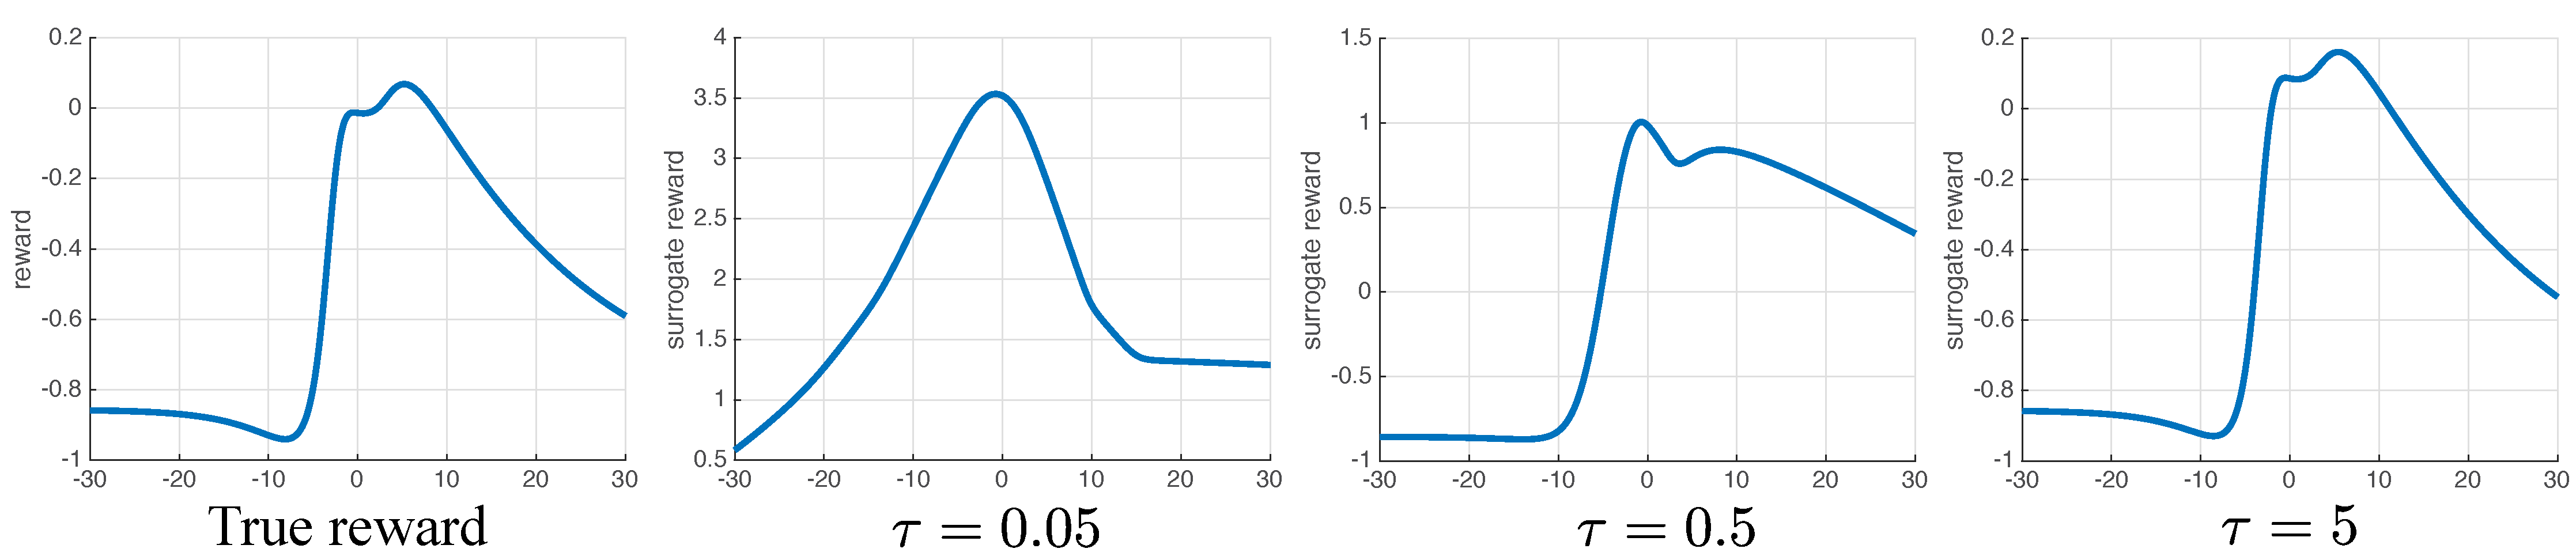
\includegraphics[width=1.0\linewidth]{./sr_simulation.pdf}
\end{center}
\caption{
Simulation results for the true reward $\pi_\theta^\top r$ and $\SR(\pi_\theta)$
with different values of $\tau$ in a bandit setting with 10,000 actions. Each action is represented by a feature $\omega\in \mathbb{R}$. Let $\Omega = \left( \omega_1, \dots, \omega_{10,000} \right)$ be the feature vector. The policy $\pi_\theta$ is parameterized by a weight scalar $\theta\in \mathbb{R}$ and defined by $\text{softmax}(\Omega^{\top}\theta)$. True reward landscape shows $\pi_\theta^\top r$ as a function of $\theta$. The rest figures show \SR($\pi_\theta$) as a function of $\theta$ with different values of $\tau$.}
\label{fig:srsimulation}
\end{figure*}
